\documentclass[11pt]{article}
\usepackage[margin=1in]{geometry}
\usepackage[usenames,dvipsnames]{xcolor}
\usepackage{amsmath,amssymb,graphicx,booktabs,microtype}
\usepackage[colorlinks=true,linkcolor=NavyBlue,citecolor=NavyBlue,urlcolor=NavyBlue]{hyperref}
\usepackage{listings}
\usepackage{caption}
\usepackage{tikz}
\usetikzlibrary{arrows.meta,positioning,calc,decorations.pathmorphing}
\captionsetup{font=small,labelfont=bf}
\usepackage[section]{placeins}
\renewcommand{\topfraction}{0.92}\renewcommand{\bottomfraction}{0.7}
\renewcommand{\textfraction}{0.08}\renewcommand{\floatpagefraction}{0.8}
\setcounter{topnumber}{3}\setcounter{totalnumber}{4}
\providecommand{\costC}{\textbf{[no data]}}
\providecommand{\etaC}{\textbf{[no data]}}
\providecommand{\etahiC}{\textbf{[no data]}}
\providecommand{\etaloC}{\textbf{[no data]}}
\providecommand{\gain}{\textbf{[no data]}}
\providecommand{\nC}{\textbf{[no data]}}
\providecommand{\slowdown}{\textbf{[no data]}}
\providecommand{\githash}{}\renewcommand{\githash}{35ca78f}
\providecommand{\pardelta}{}\renewcommand{\pardelta}{2.303}
\providecommand{\parfdisc}{}\renewcommand{\parfdisc}{10}
\providecommand{\parassoc}{}\renewcommand{\parassoc}{100}
\providecommand{\parkoffR}{}\renewcommand{\parkoffR}{900}
\providecommand{\parkoffW}{}\renewcommand{\parkoffW}{9000}
\providecommand{\parkcat}{}\renewcommand{\parkcat}{100}
\providecommand{\parkunR}{}\renewcommand{\parkunR}{0.05}
\providecommand{\parkpfR}{}\renewcommand{\parkpfR}{5.549}
\providecommand{\parkpfW}{}\renewcommand{\parkpfW}{55.49}
\providecommand{\parkligc}{}\renewcommand{\parkligc}{2.542e-06}
\providecommand{\parvcom}{}\renewcommand{\parvcom}{11.1}
\providecommand{\pardrive}{}\renewcommand{\pardrive}{20}
\providecommand{\parconc}{}\renewcommand{\parconc}{1000}
\providecommand{\parnchains}{}\renewcommand{\parnchains}{200}
\providecommand{\parpfratio}{}\renewcommand{\parpfratio}{0.5}
\providecommand{\parkon}{}\renewcommand{\parkon}{0.1}
\providecommand{\parkchemo}{}\renewcommand{\parkchemo}{500}
\providecommand{\lsdEoneR}{}\renewcommand{\lsdEoneR}{2.197}
\providecommand{\lsdEoneW}{}\renewcommand{\lsdEoneW}{4.5}
\providecommand{\lsdEtwoR}{}\renewcommand{\lsdEtwoR}{-5.404}
\providecommand{\lsdEtwoW}{}\renewcommand{\lsdEtwoW}{-3.101}
\providecommand{\lswomegazeroone}{}\renewcommand{\lswomegazeroone}{100}
\providecommand{\lswomegaonetwo}{}\renewcommand{\lswomegaonetwo}{1.111}
\providecommand{\lswomegatwozero}{}\renewcommand{\lswomegatwozero}{2.542e-06}
\providecommand{\lsdeltatwoone}{}\renewcommand{\lsdeltatwoone}{2.303}
\providecommand{\etaeq}{}\renewcommand{\etaeq}{0.09091}
\providecommand{\etahop}{}\renewcommand{\etahop}{0.01}
\providecommand{\etairr}{}\renewcommand{\etairr}{0.09091}
\providecommand{\etaB}{}\renewcommand{\etaB}{0.101}
\providecommand{\etaloB}{}\renewcommand{\etaloB}{0.0986}
\providecommand{\etahiB}{}\renewcommand{\etahiB}{0.104}
\providecommand{\nB}{}\renewcommand{\nB}{11\,097}
\providecommand{\vB}{}\renewcommand{\vB}{9.75}
\providecommand{\costB}{}\renewcommand{\costB}{0}
\providecommand{\evB}{}\renewcommand{\evB}{700}
\providecommand{\thB}{}\renewcommand{\thB}{0.099}
\providecommand{\etaCz}{}\renewcommand{\etaCz}{0.494}
\providecommand{\etaloCz}{}\renewcommand{\etaloCz}{0.493}
\providecommand{\etahiCz}{}\renewcommand{\etahiCz}{0.496}
\providecommand{\nCz}{}\renewcommand{\nCz}{109\,234}
\providecommand{\vCz}{}\renewcommand{\vCz}{1.55e+03}
\providecommand{\costCz}{}\renewcommand{\costCz}{0.0178}
\providecommand{\evCz}{}\renewcommand{\evCz}{400}
\providecommand{\thCz}{}\renewcommand{\thCz}{0.493}
\providecommand{\slopeB}{}\renewcommand{\slopeB}{-0.761}
\providecommand{\slopethB}{}\renewcommand{\slopethB}{-0.794}
\providecommand{\slopeC}{}\renewcommand{\slopeC}{-1.57}
\providecommand{\slopethC}{}\renewcommand{\slopethC}{-1.63}
\providecommand{\prefac}{}\renewcommand{\prefac}{1.92}
\providecommand{\drivecross}{}\renewcommand{\drivecross}{5.43}
\providecommand{\etaCtheory}{}\renewcommand{\etaCtheory}{0.0183}
\providecommand{\etaBtheory}{}\renewcommand{\etaBtheory}{0.099}
\providecommand{\vCtheory}{}\renewcommand{\vCtheory}{4.13}
\providecommand{\vBtheory}{}\renewcommand{\vBtheory}{9.95}
\providecommand{\sloperatio}{}\renewcommand{\sloperatio}{2.07}
\providecommand{\etafloor}{}\renewcommand{\etafloor}{0.00826}
\providecommand{\etaBsq}{}\renewcommand{\etaBsq}{0.0098}
\providecommand{\astall}{}\renewcommand{\astall}{0.905}
\providecommand{\etaCstall}{}\renewcommand{\etaCstall}{0.0109}
\providecommand{\stallratio}{}\renewcommand{\stallratio}{1.12}
\providecommand{\vstall}{}\renewcommand{\vstall}{0.019}
\providecommand{\njobs}{}\renewcommand{\njobs}{10}
\providecommand{\nevents}{}\renewcommand{\nevents}{4.3}


\definecolor{kappakw}{HTML}{1F4E79}
\definecolor{kappacm}{HTML}{6B7B8B}
\lstdefinestyle{ka}{
  basicstyle=\ttfamily\footnotesize, breaklines=true, columns=fullflexible,
  commentstyle=\color{kappacm}\itshape, keywordstyle=\color{kappakw}\bfseries,
  morecomment=[l]{//}, morekeywords={\%init,\%obs,\%var,\%agent},
  literate={->}{{$\rightarrow$}}2 {<->}{{$\leftrightarrow$}}2,
  frame=single, rulecolor=\color{black!25}, framesep=4pt, xleftmargin=2pt,
}
\lstdefinestyle{sh}{basicstyle=\ttfamily\footnotesize,breaklines=true,
  frame=single,rulecolor=\color{black!25},framesep=4pt,columns=fullflexible}

\newcommand{\kB}{k_\mathrm{B}}
\newcommand{\ka}[1]{\texttt{#1}}

\title{\vspace{-2.2em}Kinetic proofreading in a minimal Kappa model of\\
template-directed polymerisation}
\author{Reproduction of Pigolotti \& Sartori, \emph{J.\ Stat.\ Phys.}\ \textbf{162}, 1167 (2016)}
\date{Commit \texttt{\githash}}

\begin{document}
\maketitle
\vspace{-1.5em}
\begin{abstract}\noindent
A minimal Kappa model of kinetic proofreading during template-directed polymerisation,
built from the three reactions --- add, commit, proofread --- and the energy landscape of
Pigolotti \& Sartori (2016).  The model uses a single agent type: a copy is a chain of
monomer agents, the terminus is a pattern rather than a piece of bookkeeping, and
proofreading genuinely shortens the copy.  Every rate is derived from the paper's
landscape parameterisation, including the reverse of the proofreading reaction, which is
fixed by detailed balance rather than set to zero; this makes the chemical drive on the
discard step a meaningful knob.  Stochastic simulation in PyKappa recovers the
phenomenon quantitatively: the error falls from $\etaB$ without the discard arc to
$\etaC$ with it, the logarithmic slope of the error against the discrimination energy
doubles from $\slopeB$ to $\slopeC$, and an \emph{undriven} discard arc makes the copy
five times \emph{less} accurate than no proofreading at all.  The Hopfield floor
$\eta_{\rm eq}^2$ is reached, but only as the growth velocity is driven to zero: at a
working point that keeps $\velfrac\%$ of the unproofread speed the error sits a factor
$\approx2$ above the floor, and this factor is shown to be a speed penalty rather than a
change of exponent.  Results are
cross-checked against two independent non-Kappa implementations and against the
equilibrium bound at stall.

\end{abstract}

\section{What has to be reproduced}

Kinetic proofreading is the claim that a copying machine can discriminate between a
right (cognate) and a wrong (non-cognate) monomer \emph{better than the equilibrium
binding free energy allows}, provided it spends free energy.  If the two monomers
differ by $\Delta$ in binding free energy, any equilibrium discrimination is bounded by
\begin{equation}
  \eta_{\rm eq}=\frac{1}{1+e^{\Delta/T}},
  \label{eq:etaeq}
\end{equation}
and Hopfield's construction reaches $\eta\sim e^{-2\Delta/T}$ by making the same
energy gap act twice: once when the monomer is selected, and once when an
already-incorporated monomer is discarded through a \emph{driven, and therefore
effectively irreversible}, side reaction.

Pigolotti and Sartori place this in a template-directed polymerisation setting and
give the general rate parameterisation \cite{ps2016}
\begin{equation}
  k_{ij}^{r}=\omega_{ij}\exp\!\Big[\frac{\Delta E_j^{r}+\mu_{ij}+\delta_{ij}}{T}\Big],
  \qquad
  k_{ij}^{w}=\omega_{ij}\exp\!\Big[\frac{\Delta E_j^{w}+\mu_{ij}}{T}\Big],
  \label{eq:rates}
\end{equation}
where $k_{ij}$ is the rate of the transition $j\!\to\! i$, $\Delta E_i^{r/w}$ are state
free energies, $\mu_{ij}$ is a non-conservative chemical driving that raises a forward
rate without raising its reverse, and $\delta_{ij}$ is a \emph{kinetic} discrimination
that lowers the barrier of the pair $\{i,j\}$ for right monomers in \emph{both}
directions.  Their Protocol~B (states $0\!\rightleftharpoons\!1\!\rightleftharpoons\!2$)
is the Michaelis--Menten-like control; Protocol~C adds a discard arc
$2\!\rightleftharpoons\!0$ and is the proofreading scheme.  The classic square law is
recovered for the specific choice
$\delta_{10}=\delta_{02}=0$, $\Delta E_2=\Delta E_1$ for each species, and
$\delta_{21}=\Delta E_2^{w}-\Delta E_2^{r}$.

Those three states and the discard arc are exactly the \emph{add} / \emph{commit} /
\emph{proofread} reactions of the sketch this work started from, and they are what the
Kappa model below encodes.

\section{The Kappa model}

\subsection{What to represent, and what not to}

The sketch shows two strands: a template, and a growing copy whose last residue can be
excised.  In the minimal reduction the template is homogeneous --- every position
accepts one cognate species and rejects one non-cognate species --- so the template
carries no information that is not already carried by the label
\emph{right}/\emph{wrong} on the incoming monomer.  Representing it explicitly would
double the agent count and the rule count without changing a single rate.  It is
therefore dropped, and what remains is one agent type:

\begin{center}\ka{M(p, n, c\{n y\}, k\{R W S\})}\end{center}

\begin{description}\itemsep2pt
\item[\ka{p}, \ka{n}] the $5'$ and $3'$ backbone sites of a residue.  A bond
  \ka{p--n} means ``these two residues occupy adjacent template positions''.
\item[\ka{c}] \ka{\{n\}}: the residue occupies the active site, base-paired to the
  template, but is not yet covalently joined (state~1).  \ka{\{y\}}: the residue has
  been committed to the copy (state~2).
\item[\ka{k}] \ka{\{R\}} cognate, \ka{\{W\}} non-cognate, \ka{\{S\}} the primer that
  nucleates a copy.
\end{description}

Two consequences are worth stating because they are what makes the model small.
First, \textbf{no polymerase agent is needed}: the $3'$ end of a copy is the unique
\ka{M(c\{y\}, n[.])} in its connected component, so ``where the machine is'' is
readable off the graph.  Second, \textbf{the provisional occupancy of the active site
is encoded as a bond plus an internal state} rather than as a separate tether.  In the
sketch the incoming monomer hangs off the template and is not yet attached to the copy;
here it is attached, but with \ka{c\{n\}}.  The two representations are isomorphic as
state machines, and the latter needs one site fewer and no extra agent.

Because the copy is a real chain of agents, a proofreading event genuinely shortens it,
and the residue it exposes becomes the new terminus and is itself proofreadable.  The
model therefore contains multi-step backtracking, which \cite{ps2016} lists as a
generalisation beyond its own core treatment.

\subsection{The rules}

Every rule below is written twice, once for $\nu=\ka{R}$ and once for $\nu=\ka{W}$;
this costs nothing and lets the two species be tallied separately.  Rates are the
base-parameter values of Table~\ref{tab:params}.

\lstinputlisting[style=ka,caption={The six reactions, for $\nu=\ka{R}$.  The
seed \ka{M(k\{S\})} has \ka{p[.]}, so it never matches the second slot of
\emph{proofread} and a copy can never be eroded past its primer.},
label={lst:rules}]{rules_R.ka}

\emph{add} ($0\!\to\!1$) and \emph{reject} ($1\!\to\!0$) are the selection step;
\emph{commit} ($1\!\to\!2$) and \emph{uncommit} ($2\!\to\!1$) are the chemistry;
\emph{proofread} ($2\!\to\!0$) is the discard arc, and \emph{ligate} ($0\!\to\!2$) is
its thermodynamic reverse.  Deleting the last two rules gives Protocol~B.

\subsection{From the landscape to the rate constants}

The parameterisation was fixed before consulting the paper's own numbers, by reading
the discrimination energies $\delta_{01},\delta_{12},\delta_{20}$ off the energy-landscape
sketch as \emph{barrier} differences --- which, because a barrier is shared by both
directions of a step, is precisely the meaning $\delta_{ij}$ has in
Eq.~\eqref{eq:rates}.  Adopting Hopfield's special case then forces:

\begin{description}\itemsep3pt
\item[$\delta_{01}=0$:] the association barrier does not discriminate, so
  $k^{\rm add}$ is the same for R and W and the whole of $\Delta_1$ sits in the
  rejection rate, $k^{\rm rej}_{W}=e^{\Delta}k^{\rm rej}_{R}$.
\item[$\delta_{21}=\Delta$:] the commitment barrier is lowered for R by exactly the
  amount by which state~1 is stabilised for R, so \textbf{$k^{\rm com}$ is identical
  for the two species}.  Chemistry does not discriminate; only selection and discard do.
\item[$\delta_{02}=0$:] the discard barrier does not discriminate either, so the whole
  of $\Delta_2$ sits in the excision rate, $k^{\rm pf}_{W}=e^{\Delta}k^{\rm pf}_{R}$,
  and the reverse (ligation) rate is species-independent.
\item[$\Delta_1=\Delta_2\equiv\Delta=\delta$:] a mismatch costs the same free energy
  whether the monomer is merely paired or already incorporated.
\end{description}

\noindent
The remaining numbers were chosen as follows.

\emph{Time unit.}  The pseudo-first-order association rate $k_{\rm on}c=\parassoc$ sets
the unit of time; only ratios matter.

\emph{$k^{\rm rej}_R/k^{\rm com}=9$.}  Energetic discrimination at the selection step is
only expressed if binding quasi-equilibrates before commitment: the realised ratio is
$(1+x)/(1+e^{\delta}x)$ with $x=k^{\rm rej}_R/k^{\rm com}$, which tends to $e^{-\delta}$
only for $x\gg1$.  The cost is $\approx4(1+x)$ elementary events per commitment, all of
them futile binding attempts.  $x=9$ realises $0.110$ against an ideal $0.100$ --- a
$10\%$ loss of discrimination for a fourfold saving in simulation cost.  This is the
single largest compromise in the parameter set and it is a compute compromise, not a
physical one.

\emph{$k^{\rm com}/k^{\rm unc}=2000$.}  Commitment is strongly exergonic, so
$\Delta E_2^{R}=\lsdEtwoR$: polymerisation runs forward on the monomer chemical
potential alone, with no help from $\mu_{02}$.  This matters, because it means the
drive on the discard step can be turned off without stalling the machine, and the
$\mu_{02}$ sweep of \S\ref{sec:drive} isolates the cost of \emph{proofreading} from the
cost of \emph{polymerising}.

\emph{$k^{\rm pf}_R=\parpfratio\,v_{\rm com}$}, where $v_{\rm com}=\parvcom$ is the rate
at which an empty site reaches state~2 through $0\!\to\!1\!\to\!2$.  This dimensionless
excision strength is the only genuinely free dial and is swept in \S\ref{sec:tradeoff}.

\emph{$\mu_{02}=\pardrive\,\kB T$}, of the order of NTP hydrolysis.

\emph{$k^{\rm lig}$ is not free.}  It is fixed by detailed balance around the cycle,
\begin{equation}
  \frac{k^{\rm lig}_\nu c}{k^{\rm pf}_\nu}=e^{(\Delta E_2^{\nu}-\mu_{02})/T},
  \label{eq:db}
\end{equation}
and the model \emph{keeps} it rather than setting it to zero by fiat.  That is what
makes $\mu_{02}$ a meaningful knob: at $\mu_{02}=0$ the discard arc satisfies detailed
balance with the monomer pool, and proofreading must stop working.  Almost every rate
in the model is thereby determined by the landscape rather than chosen; the function
\ka{landscape()} in \ka{kpr/model.py} inverts the rate table back to
$(\Delta E_i^{\nu},\omega_{ij},\delta_{ij},\mu_{02})$ and reproduces all twelve rates to
machine precision, which is the check that Eq.~\eqref{eq:rates} really is being obeyed.

\begin{table}[t]\centering\small
\caption{Base parameter set.  Rates are in an arbitrary time unit fixed by
$k_{\rm on}c$; energies are in units of $\kB T$.  The lower block is the
Pigolotti--Sartori landscape of Eq.~(2) recovered from the rate table by
\texttt{landscape()}, which reproduces every rate to machine precision.}
\label{tab:params}
\begin{tabular}{llll}\toprule
symbol & value & unit & how it was chosen \\ \midrule
$\delta=\Delta_1=\Delta_2$ & 2.303 & $\kB T$ & discrimination free energy; $e^{\delta}=10$ \\
$\mu_{02}$ & 20 & $\kB T$ & drive on the discard step (fuel) \\
$k^{\rm add}_{R}=k^{\rm add}_{W}=k_{\rm on}c$ & 100 & t$^{-1}$ & $\delta_{01}=0$: association does not discriminate \\
$k^{\rm rej}_{R}$ & 900 & t$^{-1}$ & rejection of a cognate monomer \\
$k^{\rm rej}_{W}$ & 9000 & t$^{-1}$ & $=e^{\delta}k^{\rm rej}_{R}$ \\
$k^{\rm com}_{R}=k^{\rm com}_{W}$ & 100 & t$^{-1}$ & $\delta_{21}=\Delta$: chemistry does not discriminate \\
$k^{\rm unc}_{R}=k^{\rm unc}_{W}$ & 0.05 & t$^{-1}$ & reverse of commitment \\
$k^{\rm pf}_{R}$ & 5.549 & t$^{-1}$ & $=\,0.5\,v_{\rm com}$, $v_{\rm com}=11.1$ \\
$k^{\rm pf}_{W}$ & 55.49 & t$^{-1}$ & $\delta_{02}=0$: $=e^{\delta}k^{\rm pf}_{R}$ \\
$k^{\rm lig}_{R}c=k^{\rm lig}_{W}c$ & 2.542e-06 & t$^{-1}$ & fixed by detailed balance, Eq.~(3) \\
$c_R=c_W$ & 1000 & copies & chemostatted free-monomer pool \\
$N_{\rm chains}$ & 200 & copies & independently growing copies \\
\midrule \multicolumn{4}{l}{\emph{implied landscape}} \\
$\Delta E_1^{R}$ & 2.197 & \multicolumn{2}{l}{ $\Delta E_1^{W}$ $=$ 4.5 } \\
$\Delta E_2^{R}$ & -5.404 & \multicolumn{2}{l}{ $\Delta E_2^{W}$ $=$ -3.101 } \\
$\omega_{01}$ & 100 & \multicolumn{2}{l}{ $\omega_{12}$ $=$ 1.111 } \\
$\omega_{02}$ & 2.54e-06 & \multicolumn{2}{l}{ $\delta_{21}$ $=$ 2.303 } \\
\bottomrule\end{tabular}\end{table}


\subsection{Keeping the monomer pool fixed}

$\eta$ depends on the ratio of free monomer concentrations, and incorporation depletes
\ka{R} roughly ten times faster than \ka{W}, so an unbuffered pool would drift the very
quantity being measured.  The pool is therefore chemostatted with a zeroth-order rule
whose rate is proportional to the deficit,
\begin{center}
\ka{. -> M(p[.], n[.], c\{n\}, k\{R\}) @ [max] (0) (\parkchemo\ * (\parconc\ - 'nfree\_R'))},
\end{center}
which pins $|\ka{M}|_{\rm free}$ to within a few parts in $10^3$ of its set point at the
working point (the free-pool counts are recorded with every run).  At low drive the
futile ligation/excision cycle consumes monomers two orders of magnitude faster, and
those conditions are run with a stiffer gain, $k_{\rm chemo}=10^5$; this costs nothing,
because the number of replenishment events equals the number of monomers consumed
whatever the gain.  The \ka{[max](0)(...)} is not cosmetic:
excision returns monomers to the pool, so the deficit can go negative and an unclamped
rate would be negative, which PyKappa propagates silently into
\ka{random.choices} as a negative weight.

\subsection{PyKappa specifics worth recording}

\begin{itemize}\itemsep1pt
\item Quoted rule labels are rejected by \ka{System.from\_ka}; rule names are carried
  alongside the generated source instead and matched back onto \ka{system.tallies}.
\item \ka{|pattern|} works inside \ka{\%var} and \ka{\%obs} but \emph{not} inside a rule
  rate: \ka{KappaTransformer} consumes the pattern subtree before
  \ka{ExpressionTransformer} sees it, and evaluation dies with
  \ka{'Pattern' object has no attribute 'type'}.  Hence the \ka{\%var} indirection in the
  chemostat rule.
\item \ka{[exp]} inside a \ka{\%var} fails to evaluate, so all Arrhenius arithmetic is
  done in Python and the resulting numbers are emitted as literals.
\item Comments must use \ka{//}; a \ka{\#} is a lexer error.
\item \ka{KappaRule.select} draws its embedding from the \emph{module-level}
  \ka{random}, not from \ka{System.rng}, so reproducibility needs \ka{random.seed()}
  as well as the \ka{seed=} argument.
\item Agent creation and deletion do work in this version, contrary to the note in the
  project's modeller skill; the chemostat depends on it.
\end{itemize}

\section{Methods}

\paragraph{Simulation.}  \parnchains{} copies grow in a common pool of \parconc{}
\ka{R} and \parconc{} \ka{W} free monomers.  Each condition is a single
continuous-time trajectory of $10^5$--$2.6\times10^6$ Gillespie events
(\nevents{}~M events over \njobs{} runs in total), sampled 500 times.  The built-in
monitor is disabled and observables are read at the sample points, because per-event
monitoring dominates the runtime.

\paragraph{Observables and statistics.}  The copy composition is read directly off the
mixture: \ka{\%obs: 'prod\_R' |M(p[\_], c\{y\}, k\{R\})|} counts cognate residues that
are part of a chain, and likewise for \ka{W}.  The error fraction is the
\emph{increment} of those counts over the last $60\%$ of a run, which discards the
transient during which chains grow from their primers; uncertainties are $1\sigma$
Wilson intervals on the corresponding binomial count.  The growth velocity is the same
increment per unit time per chain.  Rule application counts (\ka{system.tallies}) give
the number of excision events per retained residue, i.e.\ the proofreading cost.

\paragraph{Two independent references.}  Because a rule-based encoding can be subtly
wrong in ways that still produce plausible curves, the Kappa results are checked against
two implementations that share no code with PyKappa (\ka{kpr/theory.py}):
\begin{enumerate}\itemsep1pt
\item a \emph{self-consistent tip process}.  Under the paper's uncorrelated-error
  ansatz, the residue exposed by an excision is \ka{W} with probability $\eta$
  independently, which closes the dynamics on six states (active-site occupancy
  $\times$ terminal-residue species).  The stationary distribution is solved exactly and
  $\eta$ is obtained by bracketing $\eta=J_W/(J_R+J_W)$.
\item a \emph{stack SSA}: a direct Gillespie simulation of the same process on an
  explicit stack of committed residues, making no ansatz --- so it also tests whether
  the ansatz itself is good.
\end{enumerate}

\begin{figure}[t]\centering
\resizebox{\textwidth}{!}{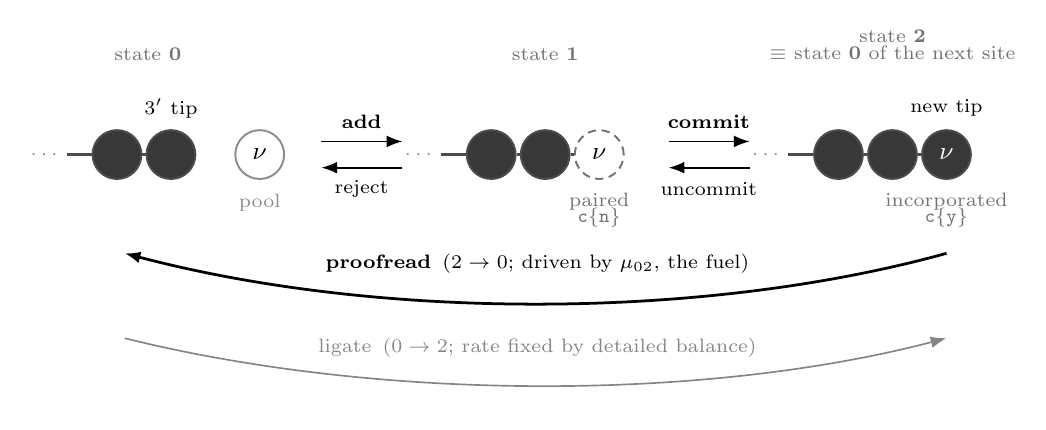
\begin{tikzpicture}[
  x=0.98cm, y=0.98cm, every node/.style={font=\small},
  res/.style={circle, draw=black!70, line width=0.7pt, minimum size=6.2mm, inner sep=0pt},
  com/.style={res, fill=black!78, text=white},
  unc/.style={res, fill=white, densely dashed, draw=black!55},
  free/.style={res, fill=white, draw=black!45},
  rr/.style={-{Latex[length=2mm]}, line width=0.6pt},
  bb/.style={line width=1.1pt, black!70},
  lbl/.style={font=\scriptsize, inner sep=1pt},
]
\newcommand{\chainbit}[1]{%
  \node[lbl,black!45] at (-0.72,0) {$\cdots$};
  \draw[bb] (-0.45,0)--(0.2,0);
  \node[com] (b#1) at (0.2,0) {};  \node[com] (c#1) at (0.9,0) {};
  \draw[bb] (b#1)--(c#1);}
% ---------------- state 0 ----------------
\begin{scope}[shift={(0,0)}]
  \node[lbl, black!55] at (0.6,1.30) {state \textbf{0}};
  \chainbit{0}
  \node[lbl] at (0.9,0.60) {$3'$ tip};
  \node[free] (f0) at (2.05,0) {$\nu$};
  \node[lbl, black!45] at (2.05,-0.62) {pool};
\end{scope}
% ---------------- 0 <-> 1 ----------------
\begin{scope}[shift={(2.85,0)}]
  \draw[rr] (0,0.17)--(1.05,0.17);   \node[lbl] at (0.52,0.42) {\textbf{add}};
  \draw[rr] (1.05,-0.17)--(0,-0.17); \node[lbl] at (0.52,-0.45) {reject};
\end{scope}
% ---------------- state 1 ----------------
\begin{scope}[shift={(4.85,0)}]
  \node[lbl, black!55] at (0.9,1.30) {state \textbf{1}};
  \chainbit{1}
  \node[unc] (d1) at (1.6,0) {$\nu$};  \draw[bb] (c1)--(d1);
  \node[lbl, align=center, black!55] at (1.6,-0.72) {paired\\[-2pt]\texttt{c\{n\}}};
\end{scope}
% ---------------- 1 <-> 2 ----------------
\begin{scope}[shift={(7.35,0)}]
  \draw[rr] (0,0.17)--(1.05,0.17);   \node[lbl] at (0.52,0.42) {\textbf{commit}};
  \draw[rr] (1.05,-0.17)--(0,-0.17); \node[lbl] at (0.52,-0.45) {uncommit};
\end{scope}
% ---------------- state 2 ----------------
\begin{scope}[shift={(9.35,0)}]
  \node[lbl, black!55, align=center] at (0.9,1.42)
       {state \textbf{2}\\[-2pt]$\equiv$ state \textbf{0} of the next site};
  \chainbit{2}
  \node[com] (d2) at (1.6,0) {$\nu$};  \draw[bb] (c2)--(d2);
  \node[lbl] at (1.6,0.60) {new tip};
  \node[lbl, align=center, black!55] at (1.6,-0.72) {incorporated\\[-2pt]\texttt{c\{y\}}};
\end{scope}
% ---------------- discard arcs ----------------
\draw[rr, line width=1.0pt]
  (10.95,-1.28) .. controls (7.8,-2.15) and (3.6,-2.15) .. (0.30,-1.28);
\node[lbl] at (5.65,-1.42) {\textbf{proofread}\, ($2\to0$; driven by $\mu_{02}$, the fuel)};
\draw[rr, black!48]
  (0.30,-2.38) .. controls (3.6,-3.20) and (7.8,-3.20) .. (10.95,-2.38);
\node[lbl, black!48] at (5.65,-2.50) {ligate\, ($0\to2$; rate fixed by detailed balance)};
\end{tikzpicture}
}
\vspace{0.6em}
\includegraphics[width=0.62\textwidth]{../figures/fig1_landscape_\githash.pdf}
\caption{\textbf{The model.}  \emph{Top:} the three reactions, as they act on the
site graph.  Filled circles are committed residues (\ka{c\{y\}}), the dashed circle is a
monomer occupying the active site but not yet incorporated (\ka{c\{n\}}); lines are
\ka{p--n} bonds.  State~2 of one incorporation is state~0 of the next, which is why
the discard reaction shortens the copy.  \emph{Bottom:} the free-energy landscape that
the rate constants of Table~\ref{tab:params} imply, obtained by inverting
Eq.~\eqref{eq:rates}.  Right (green) and wrong (red) differ by $\Delta=\pardelta\,\kB T$
in both wells; the association barrier and the discard barrier are common
($\delta_{01}=\delta_{02}=0$) and the commitment barrier is lowered for R by exactly
$\delta_{21}=\Delta$, so that commitment itself does not discriminate.  Barrier levels
are defined up to the choice of time unit.}
\label{fig:model}
\end{figure}

\section{Results}

\subsection{Proofreading squares the error}

Figure~\ref{fig:main} compares three machines that differ only in the presence and the
driving of the discard arc.  Protocol~B, with no discard arc at all, incorporates a
mismatch with probability $\etaB$ (\etaloB--\etahiB, $\nB$ residues), essentially the
equilibrium bound $\eta_{\rm eq}=\etaeq$ of Eq.~\eqref{eq:etaeq}: the selection step
alone cannot do better than the binding free energy allows.  Adding the discard arc and
driving it with $\mu_{02}=\pardrive\,\kB T$ lowers the error to $\etaC$
(\etaloC--\etahiC, $\nC$ residues), a factor of $\gain$, and brings it to within
$\approx2\times$ of the zero-speed floor $\eta_B^2=\etaBsq$ (\S\ref{sec:tradeoff}).  The middle case is the
instructive one: the discard arc is present but \emph{undriven}, and the error is
$\etaCz$ --- five times \emph{worse} than doing nothing.  At $\mu_{02}=0$,
Eq.~\eqref{eq:db} makes the reverse of proofreading fast, and ligation is a
non-discriminating route straight from state~0 to state~2 that bypasses selection
altogether.  A discard reaction is not a proofreading reaction; a \emph{driven} discard
reaction is.

\begin{figure}[t]\centering
\includegraphics[width=\textwidth]{../figures/fig2_main_\githash.pdf}
\caption{\textbf{Proofreading at work.}  (a) mismatches against residues incorporated,
for the three machines; the slope is the error fraction.  Grey guides are the
equilibrium bound $\eta_{\rm eq}$ (dashed) and the zero-speed floor $\eta_{\rm eq}^2$
(dotted).  (b) the running error
fraction converges to its steady-state value over the run.  (c) steady-state error with
$1\sigma$ Wilson intervals; black dashes are the self-consistent theory, computed with
no fitted parameter.}
\label{fig:main}
\end{figure}

\subsection{Accuracy is bought with dissipation}
\label{sec:drive}

Sweeping the drive on the discard step alone (Fig.~\ref{fig:drive}) separates the cost
of proofreading from the cost of polymerising, because in this parameterisation
polymerisation is already exergonic at $\mu_{02}=0$.  The error falls monotonically
from $\eta\approx0.49$ at zero drive to a plateau above
$\mu_{02}\approx8\,\kB T$; it does not beat the no-proofreading machine until
$\mu_{02}\approx\drivecross\,\kB T$.  This is the quantitative content of the statement
that proofreading needs fuel: the discard arc buys accuracy only once it is driven hard
enough that its reverse is negligible, and it costs both speed and monomers.
Panel~(b) shows the price: on the plateau the copy grows $\slowdown\times$ more slowly
than the no-proofreading machine, and more than two orders of magnitude more slowly than
at $\mu_{02}=0$, where the discard arc runs backwards as a fast unselective ligation.
Each retained residue costs $\costC$ excision events at the working point.

\begin{figure}[t]\centering
\includegraphics[width=\textwidth]{../figures/fig3_drive_\githash.pdf}
\caption{\textbf{The discard arc only works when it is driven.}  (a) error fraction and
(b) growth velocity against $\mu_{02}$, with everything else held at
Table~\ref{tab:params}.  Points are PyKappa, lines the self-consistent theory.  The
dashed grey line is protocol~B, the dotted line the zero-speed floor $\eta_{\rm eq}^2$.}
\label{fig:drive}
\end{figure}

\subsection{The signature: the exponent doubles}

A factor of a few in $\eta$ is not by itself evidence of proofreading --- many things
lower an error rate.  The signature of \emph{kinetic} proofreading is that the same
discrimination energy is used twice, so $\ln\eta$ falls twice as fast with $\delta$.
Figure~\ref{fig:square} sweeps $\delta$ over a factor of $\sim\!10$ in $e^{\delta}$ and
fits $\mathrm{d}\ln\eta/\mathrm{d}\delta$.  Protocol~B gives $\slopeB$; protocol~C gives
$\slopeC$, a ratio of $\sloperatio$.  (Neither is exactly $-1$ or $-2$ because
$\eta_{\rm eq}=1/(1+e^{\delta})$ itself flattens at small $\delta$; the reference curves
plotted are $\eta_{\rm eq}$ and $\eta_{\rm eq}^2$, and the \emph{ratio} of the slopes is
the parameterisation-free statement.)  Panel~(b) plots one against the other directly:
$\eta_C\approx\prefac\,\eta_B^{2}$ across the whole range.  That is the square law, with
a prefactor of order two whose origin is the subject of the next section.

\begin{figure}[t]\centering
\includegraphics[width=\textwidth]{../figures/fig4_squarelaw_\githash.pdf}
\caption{\textbf{The error is squared.}  (a) $\eta$ against the discrimination energy
$\delta$ for both protocols, with the equilibrium bound $\eta_{\rm eq}$ and its square
for reference; the fitted logarithmic slopes are quoted.  (b) the same data as $\eta_C$
against $\eta_B$, compared with $\eta_B^2$ and $2\eta_B^2$.}
\label{fig:square}
\end{figure}

\subsection{The Hopfield floor is a zero-speed limit}
\label{sec:tradeoff}

The floor $\eta_{\rm eq}^2$ assumes the discard step wins every race against commitment
of the \emph{next} residue.  In a polymer that is not free.  Write
$a=k^{\rm pf}_{R}/v_{\rm com}$ for the dimensionless excision strength.  A committed
residue survives with probability
$s_\nu=v_{\rm com}/(v_{\rm com}+k^{\rm pf}_{\nu})$, so the second discrimination factor is
\begin{equation}
  \frac{s_W}{s_R}=\frac{1+a}{1+e^{\delta}a}\;\xrightarrow[a\to\infty]{}\;e^{-\delta},
  \label{eq:stage2}
\end{equation}
but the terminus performs a biased random walk --- commitment lengthens the copy,
excision shortens it --- so net synthesis puts a ceiling on $a$.  For the base parameter
set the machine stalls at $a^{*}\approx\astall$.

Figure~\ref{fig:tradeoff} sweeps $a$ up to that ceiling.  The error falls monotonically
and, as $a\to a^{*}$ and the velocity collapses, converges on $\eta=\etaCstall$.  The
relevant floor is the square of the \emph{achieved} single-stage error,
$\eta_B^2=\etaBsq$ (slightly above the ideal $\eta_{\rm eq}^2=\etafloor$, because the
finite ratio $k^{\rm com}/k^{\rm rej}$ leaves a little first-stage discrimination on the
table); the ratio at stall is $\stallratio$.  The model therefore does reach the paper's
$\eta_{\rm min}(v\to0)=\eta_{\rm eq}^{2}$, but only at vanishing growth rate.  Everywhere
else there is a price.  At the operating point used throughout, $a=\parpfratio$, the copy
still grows at $\velfrac\%$ of the protocol-B velocity and the error is $\prefac\times$ the
floor.  The $\delta$ sweep of Fig.~\ref{fig:square} shows that this factor is nearly
constant in $\delta$: \textbf{running the machine at finite speed costs a prefactor, not
an exponent.}  The third currency is in the colour axis of
Fig.~\ref{fig:tradeoff}(a) --- excised monomers per residue retained --- and it diverges
as $a\to a^{*}$, because near stall the copy is repeatedly unmade and remade.

This is a property of proofreading \emph{embedded in polymerisation} rather than of
Hopfield's isolated enzyme, where discarding an intermediate destroys no work already
done: here every excision undoes a completed incorporation, which is why accuracy and
growth are in direct competition.

\begin{figure}[t]\centering
\includegraphics[width=\textwidth]{../figures/fig5_tradeoff_\githash.pdf}
\caption{\textbf{Speed, accuracy and cost.}  (a) error against growth velocity as the
excision strength $a=k^{\rm pf}_R/v_{\rm com}$ is varied (labels), coloured by the number
of excision events per residue retained; triangles near stall are the stack SSA, which is
far cheaper than PyKappa in that regime.  (b) the same sweep against $a$, with the
velocity on the right axis.  The error approaches the zero-speed floor $\eta_{\rm eq}^2$
only as the machine stalls.}
\label{fig:tradeoff}
\end{figure}

\subsection{Validation}

Figure~\ref{fig:valid}(a) puts every condition on a parity plot against the
self-consistent theory, together with the stack SSA.  Across all $\nruns$ conditions and
a factor of $\sim\!40$ in $\eta$, the median relative deviation of PyKappa from the
theory is $\medreldev\%$, and the deviations in units of their own binomial error are
distributed with r.m.s.\ $\rmsz$ and a worst case of $\maxz$ --- i.e.\ they are
statistical, not systematic (the small positive mean, $\meanz$, is consistent with the
$\sim\!0.3\%$ asymmetry the one-sided chemostat leaves in $c_W/c_R$).  That is the
evidence that the Kappa encoding --- in particular the decision to represent active-site
occupancy as a bond plus an internal state, and the derived ligation rate --- is doing
what it is supposed to.  The agreement
of the stack SSA with the theory additionally says that the paper's uncorrelated-error
ansatz is accurate here, i.e.\ that proofreading does not induce appreciable correlations
along the copy.

Panel~(b) is a thermodynamic check that the model cannot pass by accident.  Reducing the
polymerisation drive towards stall (by raising $k^{\rm unc}$, i.e.\ making commitment
less exergonic) must drive the error to the equilibrium bound
$\eta_{\rm eq}=1/(1+e^{\delta})=\etaeq$ \emph{whatever} the kinetics, and it does.  Any
rate that violated detailed balance would show up here as an error that undershoots or
overshoots $\eta_{\rm eq}$ at $v\to0$.

\begin{figure}[t]\centering
\includegraphics[width=\textwidth]{../figures/fig6_validation_\githash.pdf}
\caption{\textbf{Three implementations, and a thermodynamic check.}  (a) simulated
$\eta$ against the self-consistent theory for every condition run.  (b) protocol~B as
the polymerisation drive is reduced towards stall (by raising $k^{\rm unc}$); the theory
converges on the equilibrium bound $\eta_{\rm eq}$, and the independent SSA agrees within
its (large, because near stall almost nothing is incorporated) counting error at every
point.}
\label{fig:valid}
\end{figure}

\section{Discussion}

The model reproduces the phenomenon and, more usefully, reproduces the three statements
that make it non-trivial.  (i)~Without a discard arc, no choice of kinetics beats the
equilibrium bound $e^{-\delta}$ --- the selection step can be tuned, but the error is
pinned (Fig.~\ref{fig:valid}b).  (ii)~With a discard arc, the same discrimination energy
is spent twice and the exponent doubles (Fig.~\ref{fig:square}).  (iii)~The doubling is
paid for in free energy: an undriven discard arc is worse than useless, because its
reverse is an unselective shortcut into the product (Fig.~\ref{fig:drive}).

Two departures from the textbook picture are worth flagging, both of them consequences
of insisting on a real polymer rather than a single enzyme turnover.

\paragraph{The floor costs all of the speed.}  Because a committed residue is protected
only once the \emph{next} residue is committed, excision races chain extension: accuracy
and growth draw on the same event.  The floor $\eta_{\rm eq}^2$ is therefore a $v\to0$
limit, and at any useful velocity the error sits a factor of $\approx2$ above it
(Eq.~\ref{eq:stage2}).  Real polymerases sidestep this with an explicit translocation
step, which protects a residue without requiring another one to be added first; adding
such a step to the Kappa model is a two-rule change and would decouple the two races.

\paragraph{Backtracking is present and is not free.}  When the terminus is excised, the
residue it exposes becomes the new terminus and is itself proofreadable, so a copy can
be eroded several residues deep.  Pigolotti and Sartori list exactly this as a
generalisation beyond their core treatment.  Here it comes for free --- the copy is a
graph, so there is nothing to add --- and it is part of why the monomer cost diverges
at large excision strength in Fig.~\ref{fig:tradeoff}(a): near stall the copy is
repeatedly unmade, and the residues that survive are increasingly drawn from the
unselective ligation route rather than from the selective one, and every excision
throws away a completed incorporation.

\paragraph{What the rule-based encoding bought.}  Very little of this model is
bookkeeping.  There is one agent type and no polymerase, because ``the terminus'' is a
pattern (\ka{M(c\{y\}, n[.])}) rather than a piece of state that has to be maintained;
excision is a two-agent rule that needs no notion of position; and multi-step
backtracking, which would be fiddly in a state-vector model, is simply what those rules
do.  The cost is performance: PyKappa runs this model at $\sim\!1.4$k events per second,
and a discriminating selection step is intrinsically wasteful in events --- roughly
$4(1+k^{\rm rej}/k^{\rm com})\approx40$ elementary events per commitment, most of them
futile binding attempts.  That, not the physics, is what set the discrimination energies
that could be reached in a sweep.

\paragraph{Caveats.}  The discrimination energies explored, $\delta\le2.8\,\kB T$, are
modest next to real replication fidelities; the statistics at the smallest errors rest on
$\sim\!10^{2}$ mismatch events and the corresponding intervals are shown.  The
uncorrelated-error ansatz is verified here rather than assumed, but only at these
parameters.  The paper's Protocols~A and~D and its regime structure in
$(\delta_{10},\delta_{21},\delta_{02})$ --- kinetic lock, induced fit --- are not explored;
this work fixes the Hopfield corner of that parameter space and varies $\delta$,
$\mu_{02}$ and the excision strength within it.

\section{Reproducing this}

Everything is in the repository at commit \texttt{\githash}; figures carry the commit
hash of the state that produced them.

\begin{lstlisting}[style=sh]
uv sync                                    # pykappa, numpy, pandas, scipy, matplotlib

uv run python kpr/model.py                 # print the base .ka source and its rates
uv run python kpr/theory.py                # self-consistent theory + stack SSA, ~20 s

uv run python kpr/experiments.py           # all 29 runs, 4-way parallel, ~2.5 h.
                                           # resumable: finished runs are skipped.
uv run python kpr/followup.py              # repeat the low-drive runs with a stiff
                                           # monomer chemostat (~20 min)
uv run python kpr/assets.py                # report listings + parameter table
uv run python kpr/macros.py                # every number quoted in the text
uv run python kpr/figures.py               # figures/*_<hash>.pdf

cd report && tectonic -X compile report.tex
./finalize.sh                              # or: the last four steps in one go
\end{lstlisting}

\noindent
\begin{tabular}{@{}p{0.34\textwidth}p{0.62\textwidth}@{}}
\ka{kpr/model.py} & the model: \ka{Params}, \ka{kappa()} (emits the \ka{.ka}
                    source), \ka{landscape()}\\
\ka{kpr/run.py} & one trajectory: seeding, sampling, summary statistics\\
\ka{kpr/experiments.py}, \ka{kpr/followup.py} & the job lists\\
\ka{kpr/theory.py} & the two non-Kappa reference implementations\\
\ka{kpr/figures.py}, \ka{kpr/macros.py}, \ka{kpr/assets.py} & report generation\\
\ka{results/*.json} & one record per run: parameters, rates, tallies, summary\\
\end{tabular}

\medskip\noindent
Individual runs are reproducible from \ka{(seed, n\_events, params)} alone; note that
PyKappa needs both \ka{random.seed(s)} and \ka{System.from\_ka(..., seed=s)} because
rule application and embedding selection use different generators.

\appendix
\section{The complete model}
\lstinputlisting[style=ka]{model_base.ka}

\begin{thebibliography}{1}
\bibitem{ps2016} S.~Pigolotti and P.~Sartori, \emph{Protocols for copying and
proofreading in template-assisted polymerization}, J.~Stat.~Phys.~\textbf{162},
1167--1182 (2016); arXiv:1601.06940.
\bibitem{hopfield} J.~J.~Hopfield, \emph{Kinetic proofreading: a new mechanism for
reducing errors in biosynthetic processes requiring high specificity},
Proc.~Natl.~Acad.~Sci.~USA \textbf{71}, 4135 (1974).
\bibitem{ninio} J.~Ninio, \emph{Kinetic amplification of enzyme discrimination},
Biochimie \textbf{57}, 587 (1975).
\end{thebibliography}


\end{document}
